\documentclass{article}
\usepackage{amsmath}
\usepackage{amssymb}
\usepackage{graphicx}
\usepackage{hyperref}
\usepackage[version=4]{mhchem}

\title{Example 7}
\date{}

\begin{document}
\maketitle

(1985 AMC) In a circle with center \(O, A D\) is a diameter, \(A B C\) is a chord, \(B O=5\) and \(\angle A B O=\wideparen{C D}=60^{\circ}\). The length of \(B C\) is\\
(A) 3\\
(B) \(3+\sqrt{3}\)\\
(C) \(5-\frac{\sqrt{3}}{2}\)\\
(D) 5\\
(E) none of the above

Solution: (D).\\
\centering
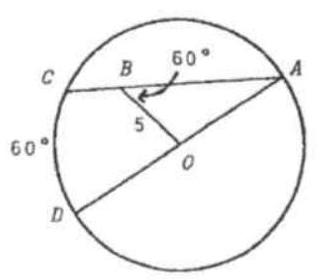
\includegraphics[width=\textwidth]{images/problem_image_1.jpg}

Since \(\wideparen{C D}=60^{\circ}, \angle B A O=30^{\circ}\). Therefore, \(\triangle A B O\) is a \(30^{\circ}-60^{\circ}-90^{\circ}\) right triangle.\\
Since \(B O=5, A O=5 \sqrt{3}, A B=10\).\\
Connect \(C D\). Since \(A D\) is the diameter, \(\triangle A D C\) is a \(30^{\circ}-\) \(60^{\circ}-90^{\circ}\) right triangle. \(A D=2 A O=10 \sqrt{3}\).\\
\(A C=\frac{\sqrt{3}}{2} \cdot 10 \sqrt{3}=15, B C=A C-A B=15-10=5\).\\
\centering
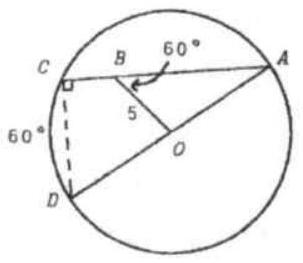
\includegraphics[width=\textwidth]{images/reasoning_image_1.jpg}


\end{document}
